% Chapter Template

\chapter{Ensayos y Resultados} % Main chapter title

\label{Chapter4} % Change X to a consecutive number; for referencing this chapter elsewhere, use \ref{ChapterX}

%----------------------------------------------------------------------------------------

En este capítulo se describen las pruebas realizadas sobre el prototipo y se explican los resultados obtenidos.

\section{Ensayos de caja negra}

Al finalizar la implementación de cada uno de los aspectos del producto, hardware, firmware y aplicación móvil, se procedió a validar los requerimientos establecidos durante la planificación. Para esto se escribió una serie de pruebas que buscaron cubrir todos los requerimientos y se las llevó a cabo, registrando el procedimiento y los resultados. Las pruebas se realizaron al terminar cada una de las etapas.

Todas las pruebas que se llevaron a cabo, especialmente las aplicadas al firmware y a la aplicación móvil, fueron del tipo ''caja negra'', es decir, fueron pruebas que buscaban comprobar que ante ciertas entradas las salidas fueran las esperadas, dejando de lado la implementación interna.

El realizar pruebas sistemáticas para comprobar los requerimientos de un producto desarrollado, representó una nueva forma de trabajo dentro de la empresa. Esto fue la causa de que se eligieran implementar pruebas de caja negra, como un primer paso en el proceso de incorporar pruebas unitarias, de integración, de sistema, etc, en los próximos proyectos que se lleven a cabo.

\section{Hardware}

El registro completo de pruebas puede encontrarse en el documento \textit{Smart Plug Hardware - Documento de pruebas} en \citep{repo_hardware}. A continuación se describen algunas pruebas significativas y se muestran sus resultados.

Al diseñar el Smart Plug se debió establecer la tensión y la corriente máxima de medición para el medidor eléctrico. Como fue explicado, estos valores se fijaron en 240VAC y 5A. por lo tanto, fue necesario validar que el hardware diseñado fuera capaz de medir estos valores.

El límite en la medición tanto de la corriente como de la tensión está impuesto por la tensión máxima de pico que soporta el front-end analógico en sus entradas diferenciales. Esta tensión no puede superar los 250mV de pico. Por lo tanto, cuando se aplicaran los valores máximos para los que fue diseñado el Smart Plug, la tensión pico en las entradas diferenciales debía estar por debajo de los 250mV.

En el caso de la tensión, se utilizó un autotransformador variable de de 0 a 250V, el cual permitió generar una tensión de 240VAC. Aplicando esta tensión, se midió la señal en la entrada diferencial del CS5490 mediante un osciloscopio, comprobándose que su tensión de pico era de 203mV, valor que se encuentra por debajo del máximo permitido por el CS5490.

En el caso de la corriente, y debido a que los canales de tensión y corriente son independientes, para producir una corriente de 5A de forma sencilla se eligió reducir la tensión con que se alimenta al Smart Plug. Para esto se utilizó el autotransformador, generando una tensión de 5VAC. Como carga se utilizó una resistencia de potencia de 1$\Omega$. Se ajustó la salida del autotransformador hasta medir una corriente de 5A sobre la carga. La tensión pico medida mediante un osciloscopio en la entrada diferencial del canal de corriente fue de 192mV, valor que comprueba que el equipo puede medir la corriente especificada.

Un aspecto que debió ser medido, aunque no estuviera relacionado con un requerimiento, fue el error relativo en las mediciones de tensión y de corriente. En las Figuras \ref{fig:error_canal_tensión} y \ref{fig:error_canal_corriente} pueden verse los resultados de las mediciones para el canal de tensión y el de corriente respectivamente.

\begin{figure}[h]
	\centering
	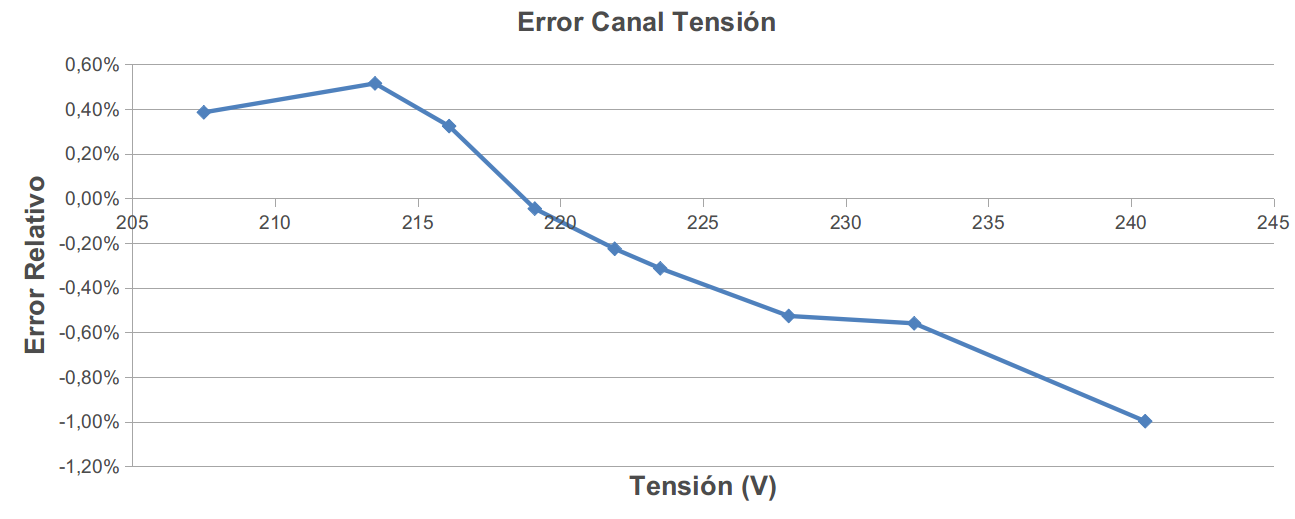
\includegraphics[width=14cm]{./Figures/4_1_1_error_canal_tension.png}
	\caption{Error relativo en el canal de tensión.}
	\label{fig:error_canal_tensión}
\end{figure}

\begin{figure}[h]
	\centering
	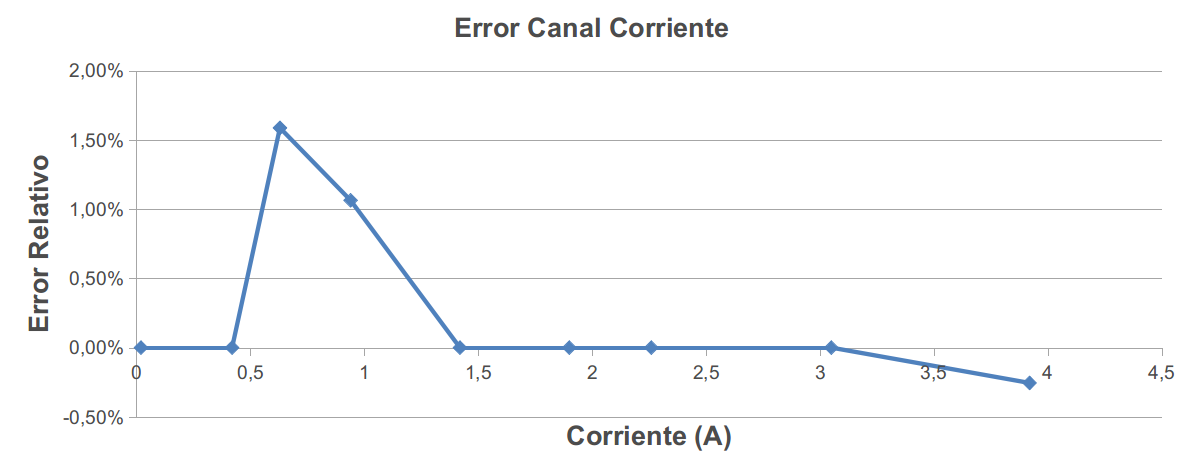
\includegraphics[width=14cm]{./Figures/4_1_1_error_canal_corriente.png}
	\caption{Error relativo en el canal de corriente.}
	\label{fig:error_canal_corriente}
\end{figure}

En el caso de la tensión, se utilizó el autotransformador variable para generar distintas tensiones de entrada y se comparó la tensión medida por el Smart Plug contra un voltímetro usado para el contraste. Como puede verse, el error relativo se encuentra por debajo del 1\% en todo el rango de tensión desde los 200VAC hasta los 240VAC.

En el caso de la corriente, se ajustó la tensión de línea sobre el Smart Plug en 10VAC utilizando el autotransformador, y se usaron distintas combinaciones de resistencias de potencia para generar diferentes corrientes. Para contrastar las mediciones se empleó un amperímetro. Los resultados se encuentran por debajo del 2\% en el rango de 0,02A hasta 4A. Los puntos en los que el error relativo está por arriba del 1\% en realidad representan una variación de una centésima en la medición respecto del amperímetro.

Para validar el resto de los requerimientos de hardware se realizaron firmwares especiales que tenían por objetivo validar un aspecto particular del equipo. Estos firmwares se pueden encontrar en \citep{repo_firmware} dentro de la carpeta \textit{Tests}. Los tests de hardware son aquellos cuyo nombre comienza con \textit{SmartPlug\_hw\_test}.


\section{Firmware}
\label{sec:validacion_firmware}

En el caso de la validación de los requerimientos del firmware, la totalidad de las pruebas se encuentran descritas en el documento \textit{Smart Plug Firmware - Documento de Pruebas v1.0} en \citep{repo_docu_firmware}.

Uno de los aspectos que se debió validar en el caso del firmware fueron las señalizaciones del led bicolor. Este led es el único medio que tiene el usuario para conocer cómo está funcionando su Smart Plug, por lo que su funcionamiento debe ser confiable. Para generar todas las señalizaciones implementadas se implementaron distintos casos de prueba en los que se simulaba la condición de funcionamiento o de falla y se observaba el resultado en el led.

A continuación se resumen las pruebas para las distintas señalizaciones:

\begin{itemize}
\item Led verde destellante a 2Hz: esta señalización se produce al iniciar el Smart Plug como un punto de acceso. Para esto, se mantuvo presionado el pulsador en la placa del Smart Plug durante 5 segundos y se comprobó que el Plug creara una red WiFi. El led comenzó a destellar con una frecuencia de 2Hz (medido con un osciloscopio) cuando se creó la red WiFi. El led dejó de destellar cuando se configuró una red WiFi a la que se tenía que conectar el Smart Plug.
\item Led verde destellante a 1Hz: esta señalización se produce mientras dura el proceso de WPS. Para producirla, se presionó el pulsador en la placa del Smart Plug. Luego de hacer esto, el led comenzó a destellar con una frecuencia de 1Hz. Se presionó el botón de WPS en un router WiFi y cuando el Smart Plug se unió a la red, el led verde dejó de destellar.
\item Led rojo destellante a 1Hz: se produce cuando el Smart Plug no puede registrarse en una red WiFi. Para producir esta situación se enciende el Smart Plug con el router WiFi desenergizado. Luego de unos segundos, al no poder conectarse a la red WiFi, el led rojo comenzó a destellar a una frecuencia de 1Hz.
\item Led verde y rojo destellan: se produce cuando el Smart Plug no puede sincronizar la su fecha y hora con un servidor NTP. Para producir esta falla, se configuró el router WiFi para que impidiera las conexiones a la dirección IP del servidor NTP usado por el Plug. Cuando se encendió el Smart Plug, luego de unos segundos el led verde y el rojo comenzaron a destellar.
\item Led verde encendido: esta señalización indica el correcto funcionamiento del Smart Plug. Para producir esta situación se eliminaron las condiciones de falla antes simuladas y el led verde se encidió luego de unos segundos.
\end{itemize}


Otro aspecto importante que debió validarse es que el Smart Plug generara un mensaje UDP periódico cada 2 segundos a la dirección de broadcast de la red WiFi. Es importante que estos mensajes existan ya que la aplicación móvil depende de estos para identificar a los Plugs existentes en la red. Además, dentro de estos mensajes periódicos debe informarse el número de ID único del dispositivo.

Para realizar la prueba se utilizó una computadora, dentro de la misma red que el Smart Plug, ejecutando un capturador de paquetes (Wireshark). En la Figura \ref{fig:mensajes_udp} puede verse una porción de la captura, en la que se aprecia que el tiempo entre mensajes UDP dirigidos a la dirección broadcast de la red es de aproximadamente 2 segundos. Además, en la misma figura se puede ver el contenido de uno de los mensajes, en donde se resaltan los seis dígitos del ID del Smart Plug (en este caso 123456) expresado en caracteres ASCII.

\begin{figure}[h]
	\centering
	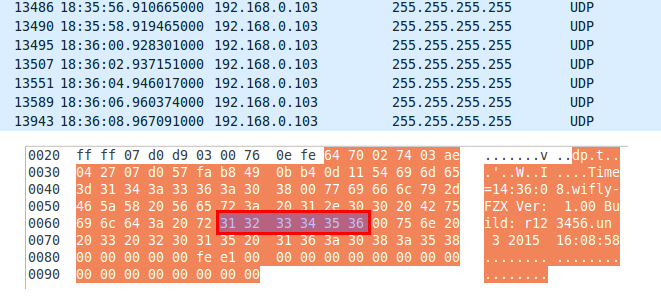
\includegraphics[width=14cm]{./Figures/4_1_2_mensajes_udp.png}
	\caption{Mensajes UDP periódicos recibidos de un Smart Plug, utilizados para identificarlo dentro de la red WiFi.}
	\label{fig:mensajes_udp}
\end{figure}


El protocolo desarrollado para comunicar los Smart Plugs con la aplicación móvil requirió ser validado completamente, probando todos los comandos y registros, para determinar si se producían las acciones esperadas y se devolvían las respuestas debidas.

Para poder conducir las pruebas sin la necesidad de desarrollar la aplicación móvil (la cual no estaba implementada al momentos de llevar a cabo la validación del firmware), se diseño e implementó una aplicación para PC que permitiera generar las tramas de acuerdo a la especificación del protocolo.

En la Figura \ref{fig:simulador_tcp} puede verse una captura del software desarrollado utilizando QT.

\begin{figure}[h]
	\centering
	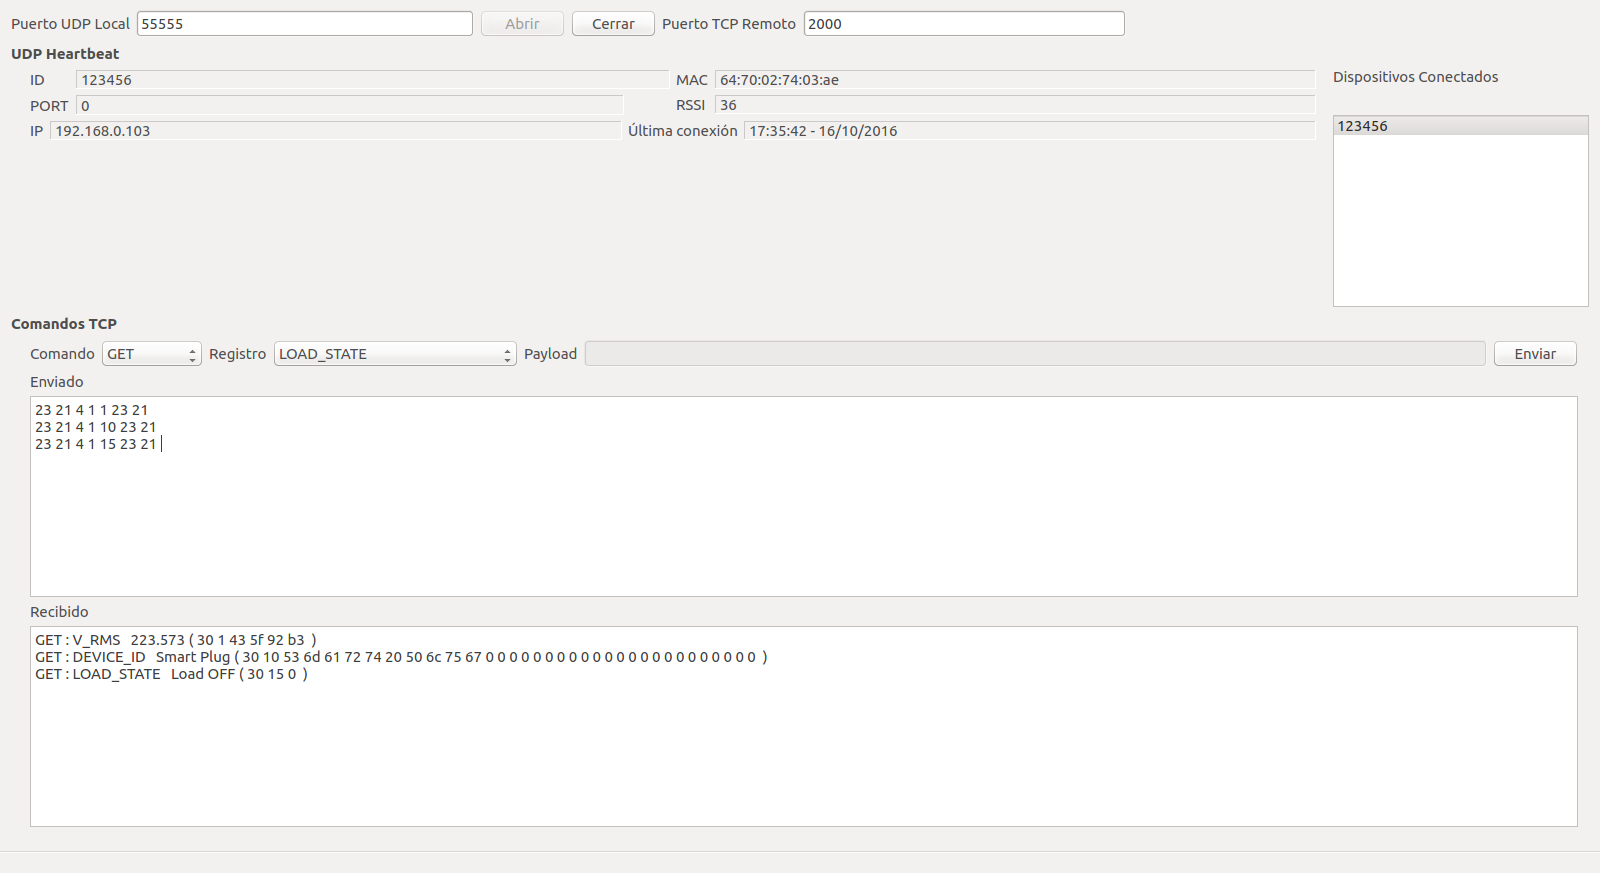
\includegraphics[width=14cm]{./Figures/4_1_2_simulador_tcp.png}
	\caption{Captura del software desarrollado que permite generar todos los comandos propuestos en el protocolo de comunicación.}
	\label{fig:simulador_tcp}
\end{figure}

La interfaz gráfica del software consta de cuatro secciones principales:

\begin{enumerate}
\item Permite elegir el puerto UDP en el que escuchar los mensajes periódicos enviados por los Smart Plugs y el puerto TCP al que mandar las tramas. Los Smart Plugs envían sus mensajes periódicos al puerto UDP 55555 y escuchan las conexiones TCP en el puerto 2000.

\item Cuando se abre el puerto UDP, se empiezan a recibir mensajes periódicos de los Smart Plugs que estén conectados en la misma red a la que pertenece la computadora que está corriendo esta aplicación. Cuando llega un mensaje periódico se agrega el ID único del Plug que lo envió en la lista de la derecha, como puede verse con el Plug de ID 123456. Al seleccionar uno de los Smart Plugs de la lista, en los controles de la izquierda de esta sección se visualizarán algunos parámetros del Plug: dirección MAC, IP, RSSI de la señal WiFi, hora de llegada del mensajes, etc.

\item Esta sección permite elegir el comando que se va a enviar al Smart Plug seleccionado en la sección 2. Se debe elegir tanto el comando como el registro afectado (en caso de que corresponda). Además, si el comando requiere un parámetro adicional, como puede ser el en el caso del comando SET, en el campo Payload se pueden ingresar los datos que debe llevar la trama.

\item Muestra la trama enviada y la trama recibida como respuesta. En el caso de la respuesta. se muestra la misma parseada de acuerdo al comando y al registro manipulado. De esta forma, por ejemplo, si se está enviando el comando GET de un registro de tipo float (como puede ser la tensión eficaz medida), la aplicación mostrará el contenido de la respuesta como un float.
\end{enumerate}

Utilizando esta aplicación se llevaron a cabo numerosos casos de prueba para comprobar la correcta implementación del protocolo en el firmware del Smart Plug. Tanto las pruebas como los resultados obtenidos pueden verse en el documento \textit{Smart Plug Firmware - Documento de Pruebas v1.0} en \citep{repo_docu_firmware}.

Por otro lado, el código fuente de esta aplicación de PC se encuentra en \citep{repo_simulador_tcp}.


\section{Aplicación móvil}

En el caso de la aplicación móvil, además de las pruebas de caja negra para validar sus requerimientos (las cuales pueden encontrarse en el documento \textit{Smart Plug App - Documento de Pruebas v1.0} en \citep{repo_docu_app}) se llevó a cabo una prueba general del sistema completo para comprobar su funcionamiento.

Básicamente la prueba general consistió en dejar conectado el Smart Plug durante 5 días con una lámpara de 60W conectada realizando distintas configuraciones para comprobar su funcionamiento.

Las acciones que se realizaron dentro de la prueba fueron:

\begin{itemize}
\item Configuración de la programación horaria para algunos días de la semana.
\item Encendido y apagado de la carga mediante la aplicación.
\item Comprobación de las mediciones eléctricas.
\item Visualización de los gráficos de potencia y energía consumida por hora.
\end{itemize}

Mediante la programación horaria se pudo comprobar que la carga se encendía y apagaba de acuerdo al día de la semana y a las horas configuradas para ese día.

Presionando el ícono asociado al Smart Plug en la lista de Plugs encontrados se pudo encender y apagar la carga.

Luego de pasados los 5 días se tenían 5 gráficos históricos de potencia y de energía consumida como se ve en la Figura \ref{fig:integracion}. En la parte derecha de la figura, puede verse uno de los gráficos de potencia promedio por hora.


\begin{figure}[h]
	\centering
	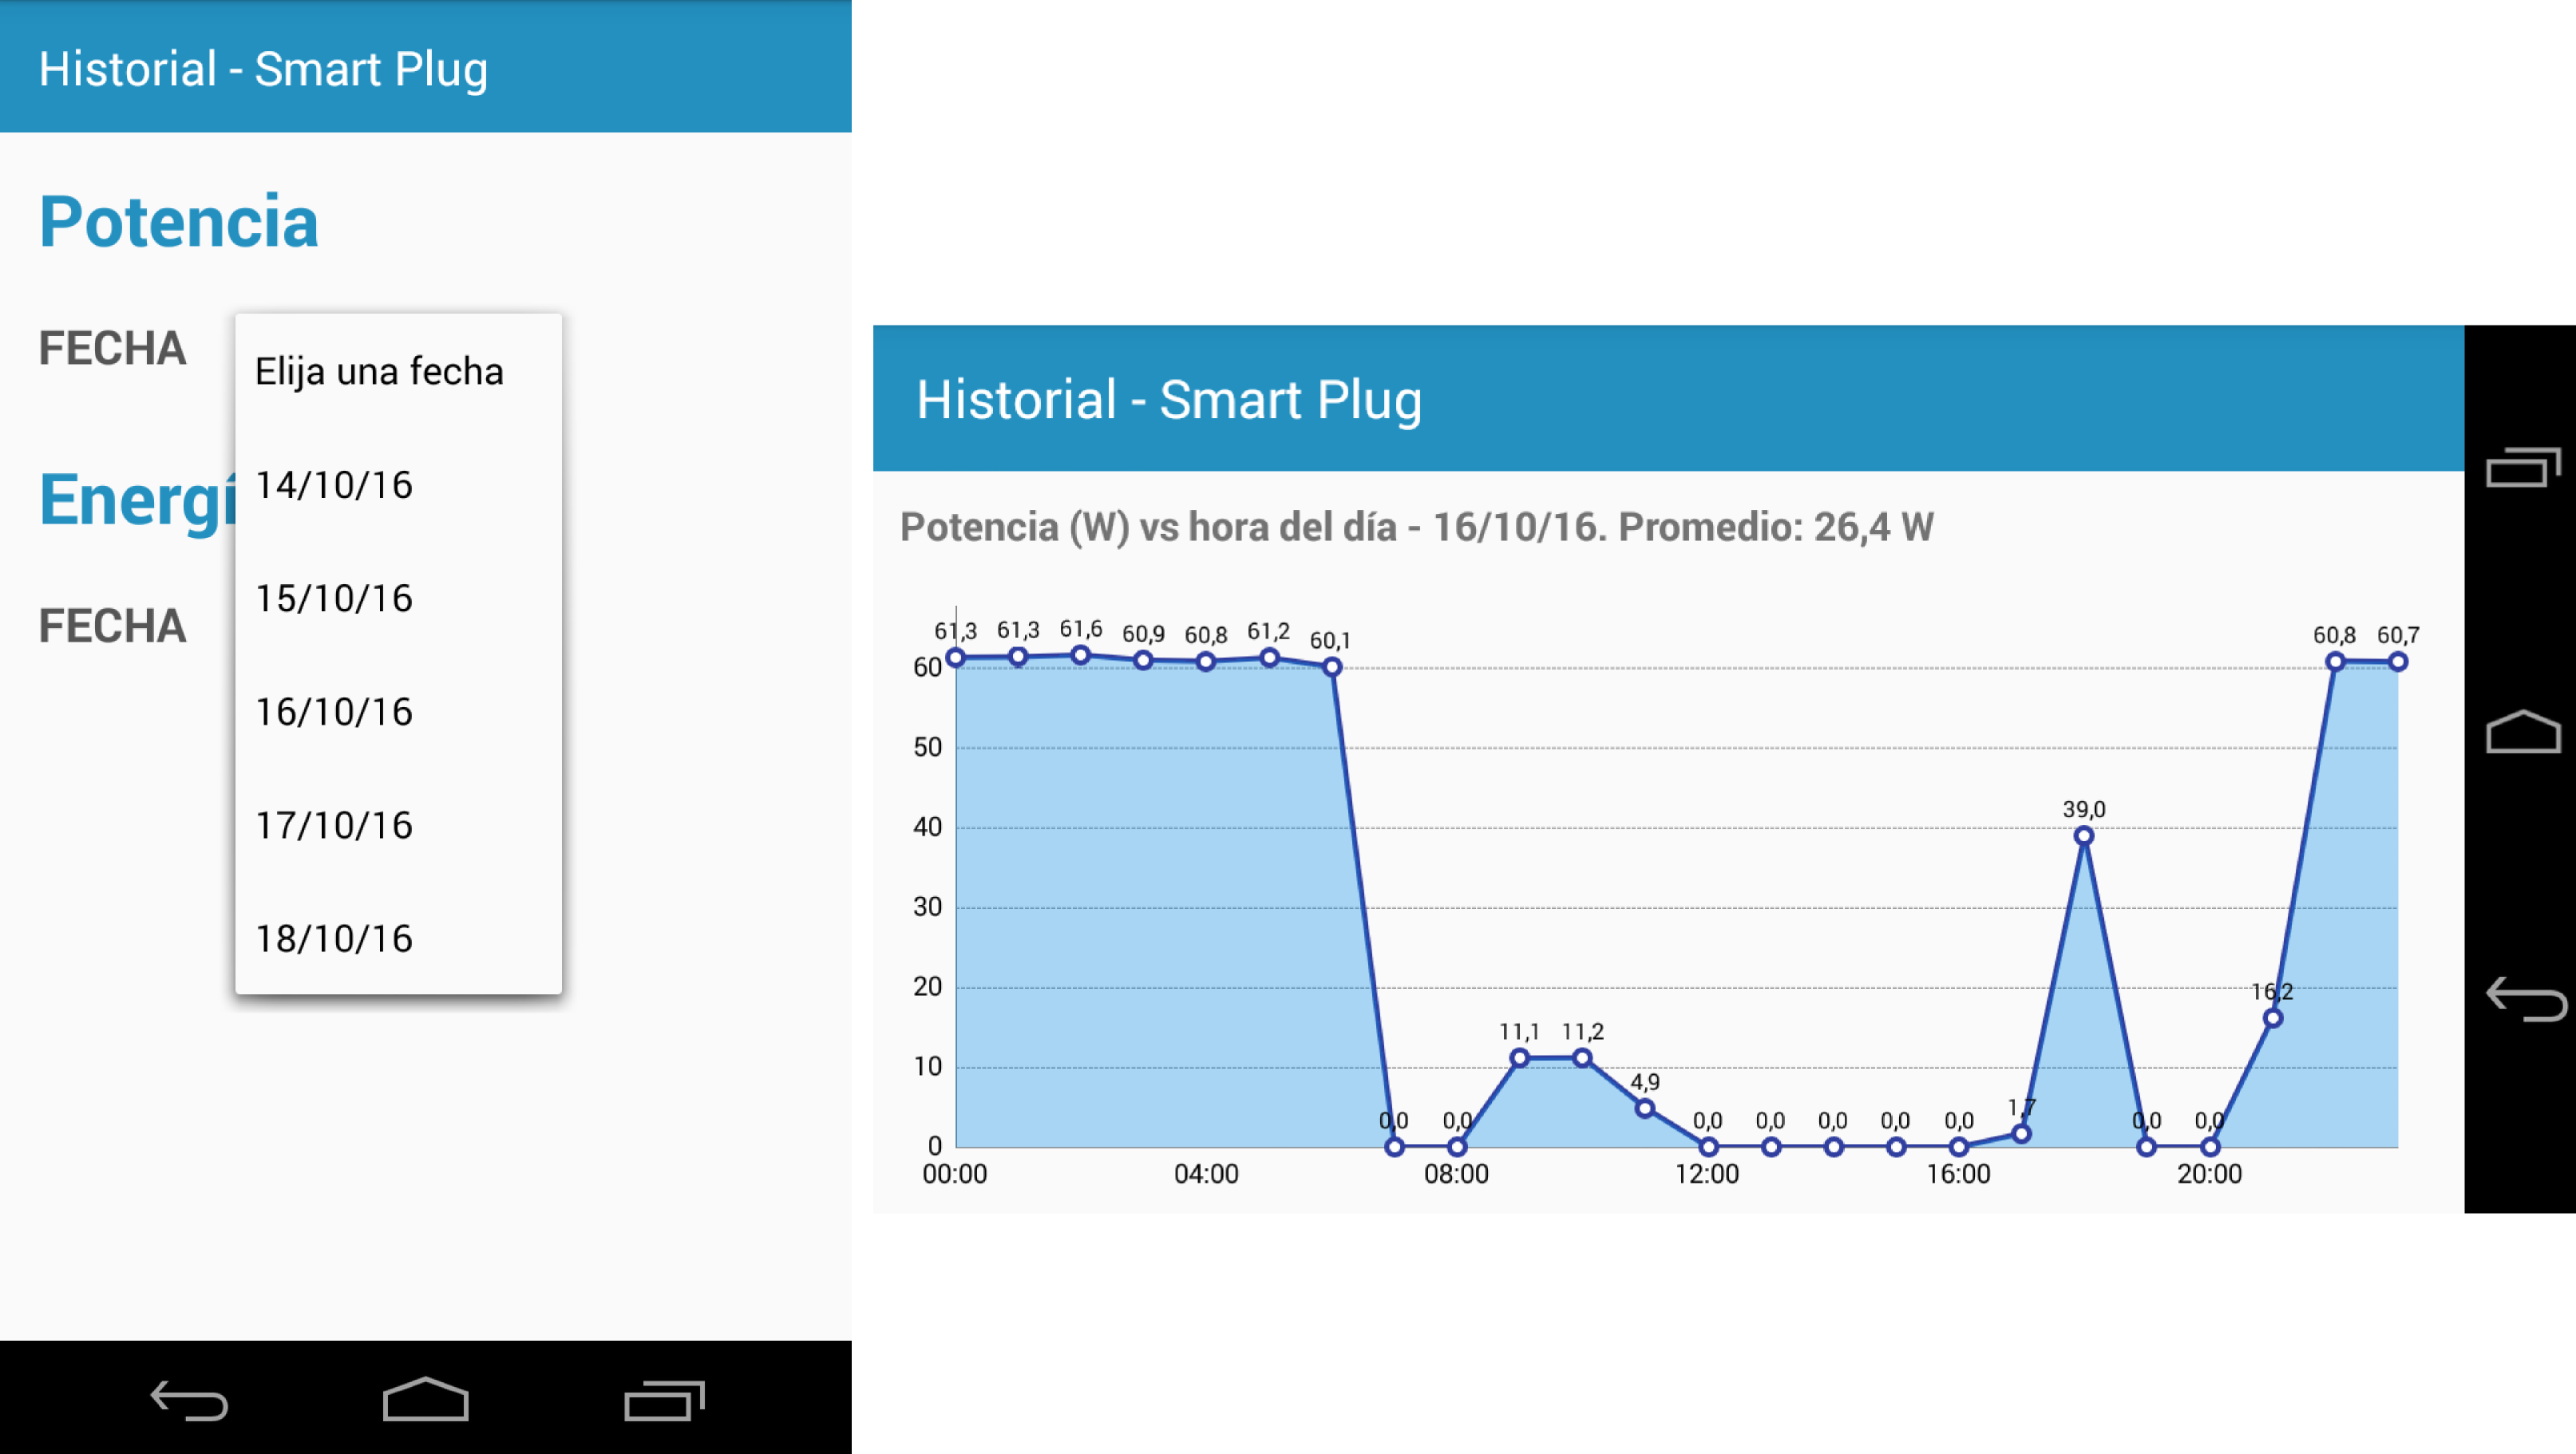
\includegraphics[width=12cm]{./Figures/4_1_3_integracion.png}
	\caption{Capturas de la aplicación móvil resultantes de la prueba de funcionamiento general del Smart Plug.}
	\label{fig:integracion}
\end{figure}